\documentclass[12pt]{article}
\usepackage[english]{babel}
%\usepackage{subcaption}
\usepackage{hyperref}
\usepackage{graphicx}
\usepackage{amsmath}
\graphicspath{{images/}}
\usepackage{geometry}
 \geometry{
 a4paper,
 total={170mm,257mm},
 left=15mm,
 top=15mm,
 }
\begin{document}
\section{Introduction} 
In this project, we have estimated the 3D motion of camera, and provided as output a plot of the trajectory of the camera. The inputs given in this project are image frames of a driving sequence taken by a camera attached in front of the car. By estimating the motion of camera. we are indirectly estimating the motion of the car using the concepts of Visual Odometry.

\section{Pipeline followed}
The following pipeline was followed to implement this project.
\subsection{Data Preparation:} The input frames were in Bayer format from which we can recover the color images using the demosaic function with GBRG alignment. That is, convert the Bayer pattern encoded image to a color image using inbuilt Opencv function:

\begin{figure}[h]
    \centering
    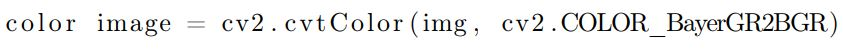
\includegraphics[width=12cm]{data1}
\end{figure}

Then we extracted the camera parameters using $ReadCameraModel.py$ file provided.
\begin{figure}[h]
    \centering
    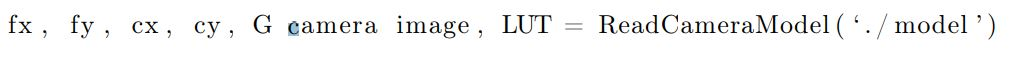
\includegraphics[width=14cm]{data2}
\end{figure}

Then we undistorted the images frames using $UndistortImage.py$ file provided.
\begin{figure}[h]
    \centering
    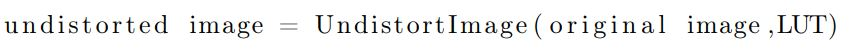
\includegraphics[width=12cm]{data3}
\end{figure}
Since, there were many image frames, for easy access and optimize the code, we converted the undistorted image sequence into a single video.

\subsection{Estimating Fundamental Matrix:}The fundamental matrix, denoted by F, is a 3x3 matrix of rank 2 that relates the corresponding set of points in two images from different views. Lets say a point $X$ in 3D is represented as $(x_i, y_i, 1)$ in camera $C1$ and $(x^{'}_i, y^{'}_i, 1)$ in camera $C2$. Fundamental matrix related these points in two different cameras using the following relation.
\newpage
\begin{figure}[h]
    \centering
    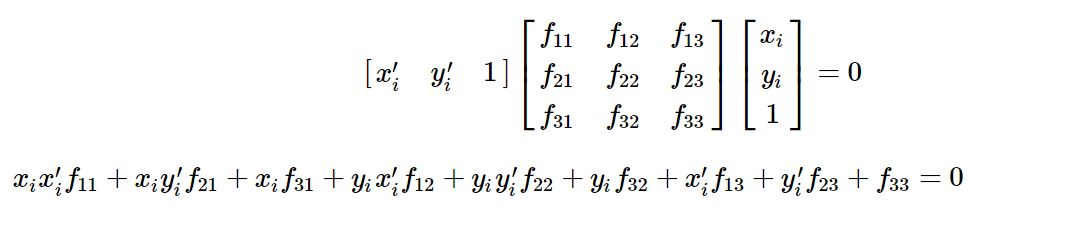
\includegraphics[width=13cm]{FM}
\end{figure}
The above equation can be modified to the matrix form $Ax = 0$
\begin{figure}[h]
    \centering
    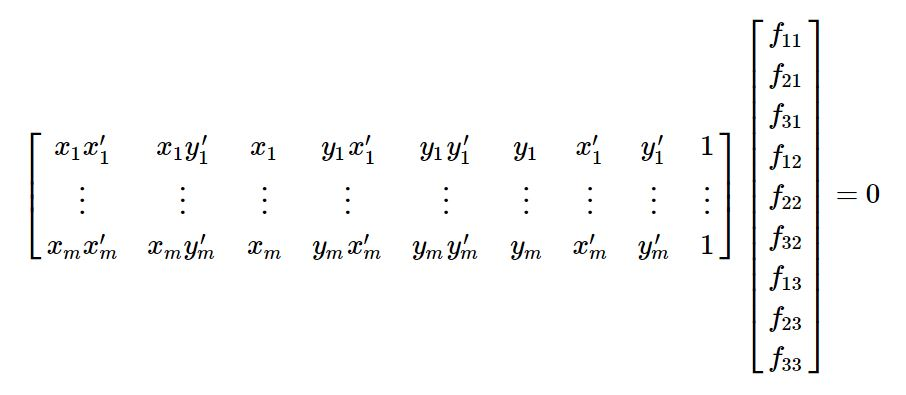
\includegraphics[width=13cm]{FM2}
\end{figure}
Hence, the fundamental matrix can be found finding the SVD of matrix A, the decomposition $U*S*V^T$ would be obtained with U and V orthonormal matrices and a diagonal matrix S that contains the singular values. The last column of V is the true solution of the matrix equation $Ax = 0$ which lies in null space of matric A. The last column of V can be reshaped into fundamental matrx of size 3x3. This is done in the python file EstimateFundamentalMatrix.py. The fundamental matrix obtained is compared with the results obtained from cv2.findFundamentalMat Opencv function which uses 8-point algorithm. The results are shown below:
\begin{figure}[h]
    \centering
    \includegraphics[width=11cm]{funmat}
    \caption{Fundamental matrix comparison}
    \label{fig:Fundamental matrix comparison}
\end{figure}
\newline
The code snippet of the comparison is shown below:
\newpage
\begin{figure}[h]
    \centering
    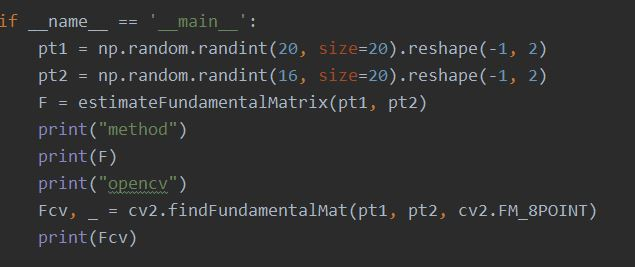
\includegraphics[width=11cm]{funcode}
    \caption{Fundamental matrix comparison code}
    \label{fig:Fundamental matrix comparison code}
\end{figure}
\subsection{Match Outlier Rejection via RANSAC:}
The corresponding point in two images computed may be noisy. Thus, we may not get the correct estimate of the fundamental matrix. So, in order to get the correct estimate, we employ RANSAC algorithm to remove the outliers. After removing the outiers, the fundamental matrix F with maximum number of inliers is chosen. The RANSAC algorithm is implemented in GetInlierRansac2.py python file. The fundamental and essential matrix obtained by implementing RANSAC algorithm is compared with results from Opencv functions like  cv2.findEssentialMat and cv2.findFundamentalMat which uses RANSAC algorithm. The following are the results obtained:
\begin{figure}[h]
    \centering
    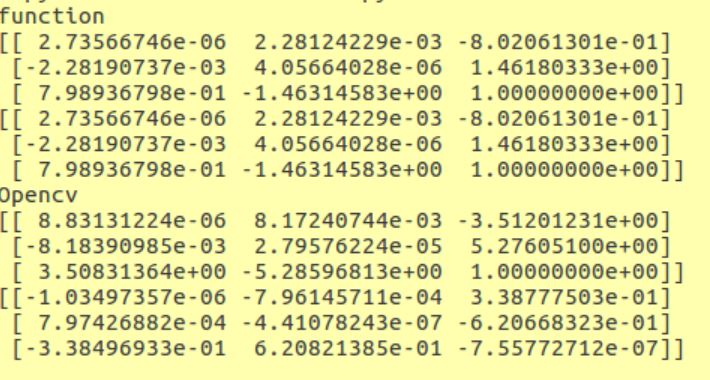
\includegraphics[width=11cm]{ransac}
    \caption{Fundamental and Essential matrix comparison RANSAC}
    \label{fig:Fundamental and Essential matrix comparison RANSAC}
\end{figure}
\newline 
The reason why the function output and the Opencv output are different is because of RANSAC algorithm does not sample the points accurately.
The code snippet is given below:
\newpage
\begin{figure}[h]
    \centering
    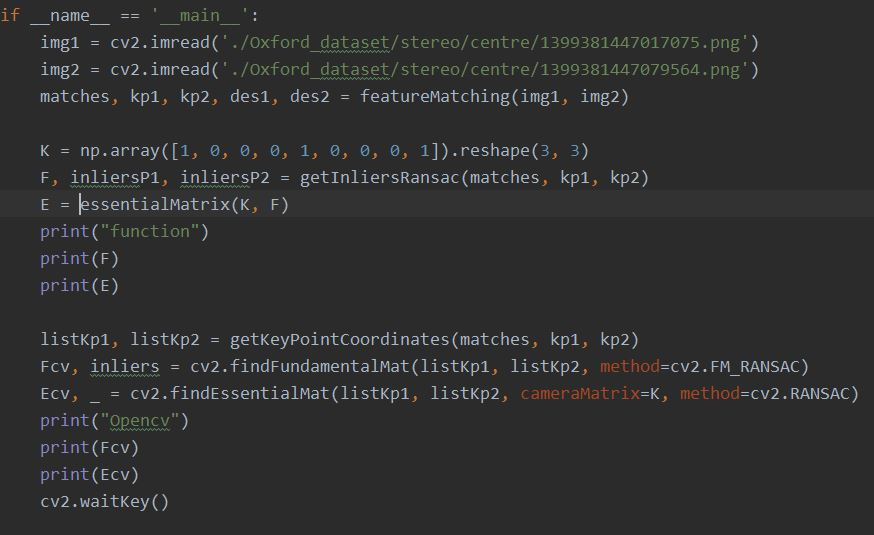
\includegraphics[width=11cm]{ransac1}
    \caption{Fundamental and Essential matrix comparison RANSAC code}
    \label{fig:Fundamental and Essential matrix comparison RANSAC code}
\end{figure}
\subsection{Estimate Essential Matrix from Fundamental Matrix:}
We can find the relative camera poses between two images using the fundamental matrix F. In order to compute relative poses between two images we need to first compute essential matrix(E). In order to compute, essential matrix, we need to intrinsic matrix(K). The relation is given by:
\begin{figure}[h]
    \centering
    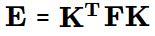
\includegraphics[width=3cm]{EM}
\end{figure}
\newline
By, due to noises present in matrix K, the third eigen value of matrix E is not zero. This can be corrected by reconstructing it with (1,1,0) singular values.
\begin{figure}[h]
    \centering
    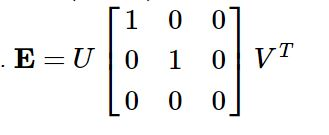
\includegraphics[width=6cm]{EM2}
\end{figure}
This is implemented in EssentialMatrixFromFundamentalMatrix.py python file. The result of the essential matrix was verified by passing the camera matrix as identity matrix and was found that both fundamental and essential matrix was equal.
\newpage
\begin{figure}[h]
    \centering
    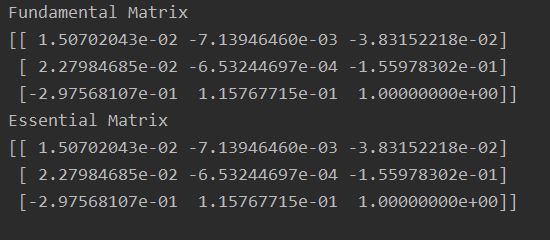
\includegraphics[width=10cm]{essmat}
    \caption{Essential matrix}
    \label{fig:Essential matrix}
\end{figure}
The code snippet of the comparison is shown below:
\begin{figure}[h]
    \centering
    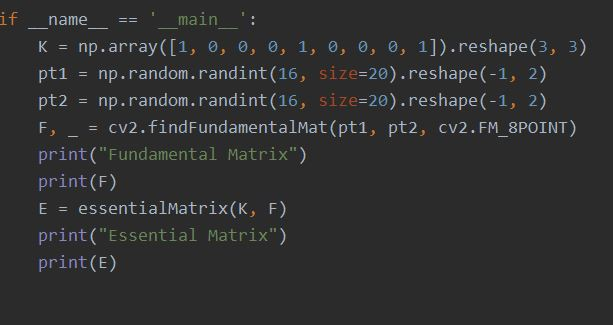
\includegraphics[width=11cm]{esscode}
    \caption{Essential matrix comparison code}
    \label{fig:Essential matrix comparison code}
\end{figure}
\subsection{Estimate Camera Pose from Essential Matrix}
Camera pose refers to the position and angle at which the camera is places w.r.t to the world coordinates. Position of the camera refers to the center of the camera. The position and rotation of the camera can be determined by using essential matrix(E). First, we compute the svd of E.
\begin{figure}[h]
    \centering
    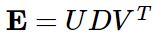
\includegraphics[width=2cm]{EM3}
\end{figure}
\newline
Then using the W matrix which is given by:
\newpage
\begin{figure}[h]
    \centering
    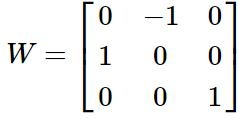
\includegraphics[width=4cm]{EM4}
\end{figure}
The camera center C and rotation of the camera R can be computes as follows:
\begin{enumerate}
\item $C_1 = U(:,3) , R_1 = U*W*V^{T}$
\item $C_2 = -U(:,3) , R_2 = U*W*V^{T}$
\item $C_3 = U(:,3) , R_3 = U*W*V^{T}$
\item $C_4 = -U(:,3) , R_4 = U*W*V^{T}$
\end{enumerate}
If the $det(R) = -1,$ the camera pose must be corrected i.e. $C=-C$ and $R=-R$. This is implemented in ExtractCameraPose.py python file. The camera pose obtained was compared with Opencv function cv2.decomposeEssentialMat function. The compared results are shown below:
\begin{figure}[h]
    \centering
    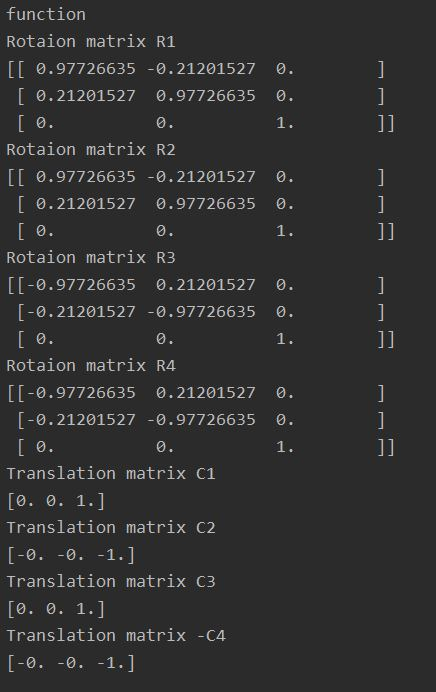
\includegraphics[width=9cm]{came}
    \caption{Pair of Rotation and Translation matrix obtained}
    \label{fig:Pair of Rotation and Translation matrix obtained}
\end{figure}
\newline
In Opencv, the function returns 2 rotation matrices(R,-R) and 1 translation matrix(T).Generally 4 possible poses exists for a given E. They are [R1, T], [R1, -T], [R2, T], [R2, -T]. These possible poses are exactly equal to the poses obtained from formula. 
\begin{enumerate}
\item  $[R, T]  ->   [R1, C_1]$
\item  $[R, -T]  ->  [R2, C_2]$
\item  $[-R, -T]  -> [R3, C_3]$
\item  $[-R, -T]  -> [R4, C_4]$
\end{enumerate}
The results are shown below:
\begin{figure}[h]
    \centering
    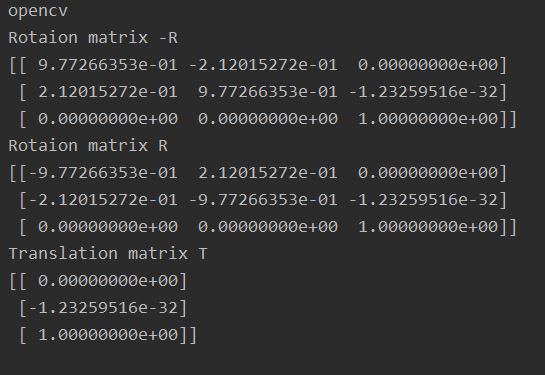
\includegraphics[width=6cm]{came1}
    \caption{Rotation and Translation matrix obtained from Opencv}
    \label{fig:Rotation and Translation matrix obtained from Opencv}
\end{figure}
\newline
The code snippet of the comparison is shown below:
\begin{figure}[h]
    \centering
    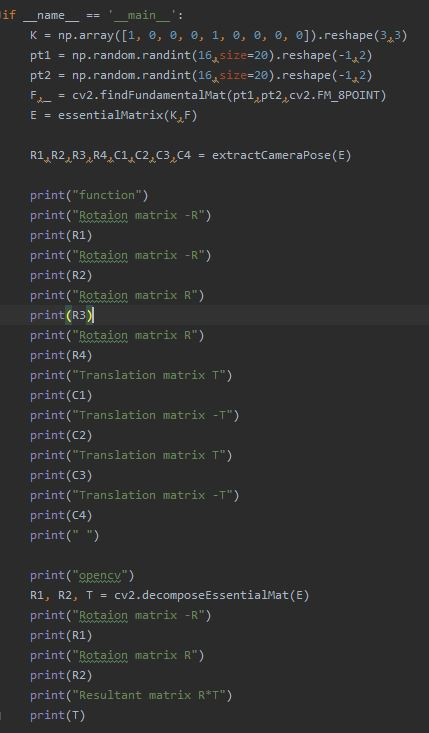
\includegraphics[width=7.5cm]{camecode}
    \caption{Rotation and Translation matrix code}
    \label{fig:Rotation and Translation matrix code}
\end{figure}
\subsection{Linear Triangulation:}
Linear triangulation is a method to extract the 3D coordinates of a point in the image frame(X) from two different camera projections of the point$(x,x^{'})$ from 2 cameras.  From the camera matrix of two cameras($C_1, C_2$) which are $P,P^{'}$, we need to estimate the 3D coordinates of X using linear triangulation. \\
We know the relation between $(x,x^{'})$ and $P,P^{'}$ and X.
\begin{equation}
	x = PX
\end{equation}
\begin{equation}
	x^{'} = P^{'}X
\end{equation}
and we also know that
\begin{equation}
	cross(x, PX)= 0 
\end{equation}
\begin{figure}[h]
    \centering
    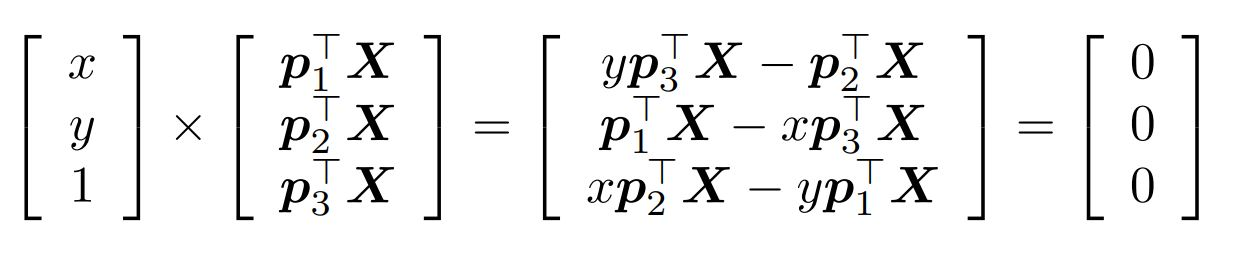
\includegraphics[width=9cm]{formula}
\end{figure}
Third line is a linear combination of the first and second lines.  So, we can remove it. So, we get:
\begin{figure}[h]
    \centering
    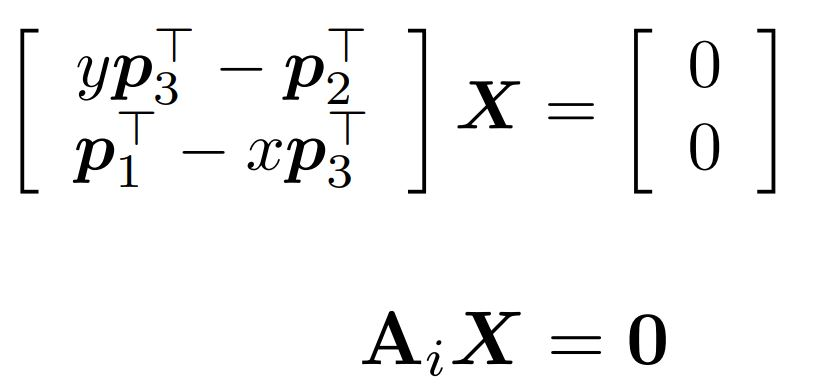
\includegraphics[width=7cm]{formula1}
\end{figure}
By concatenating points from two images, we get:
\begin{figure}[h]
    \centering
    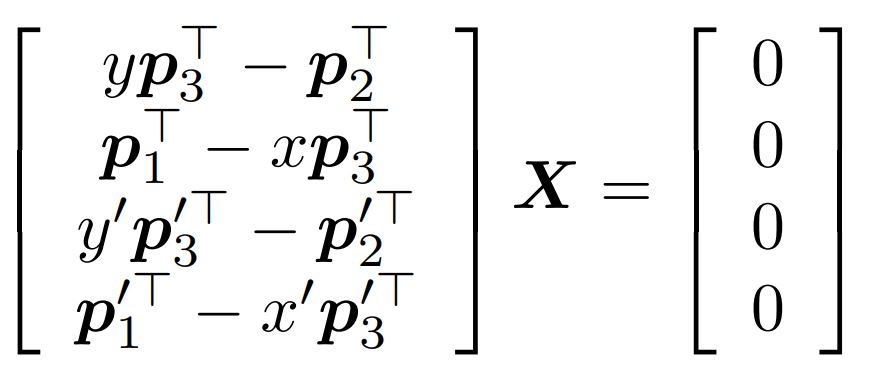
\includegraphics[width=5cm]{formula2}
\end{figure}
This is a system of homogenous linear equation of the form $Ax = 0$. The solution is obtained using svd. The goal is to minimize the error caused due to noise. So, we find the total least square approach to minimize the error. So, the solution is the eigen vector with least eigen value of $A^{T}*A$. This is implemented in LinearTriangulation.py python file.

\subsection{Triangulation Check for Cheirality Condition}
After getting the 3D coordinates from linear triangulation, we need to check whether the obtained point is in front or behind the camera. We always want our point to be in front of the camera. This is checked by using Cheirality condition. Cheirality condition checks the sign of the depth in the camera coordinate w.r.t camera center. The condition is given by:
\begin{equation}
r_3(X - C) > 0
\end{equation}
where $r_3$ is the third row of the rotation matrix.The best camera configuration, (C,R,X) is the one that produces the maximum number of points satisfying the cheirality condition. This is implemented in DisambiguateCameraPose.py python file.

\subsection{Plotting the motion of the camera:}
The final part of this pipeline is plotting the camera center based on translation and rotation between successive frames.
\begin{figure}[h]
    \centering
    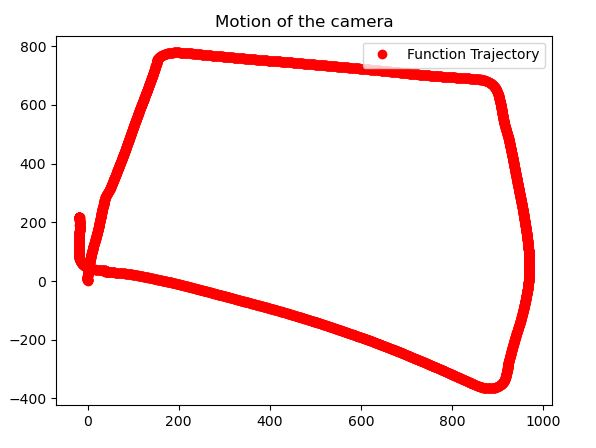
\includegraphics[width=11cm]{output1}
    \caption{Camera Trajectory}
    \label{fig:Camera Trajectory}
\end{figure}

\section{Comparison:(Extra credit)}
The comparison is made by plotting the trajectory obtained from our method and using opencv functions like cv2.findEssentialMat and cv2.recoverPose. The results of the comparison are shown below:
\begin{figure}[h]
    \centering
    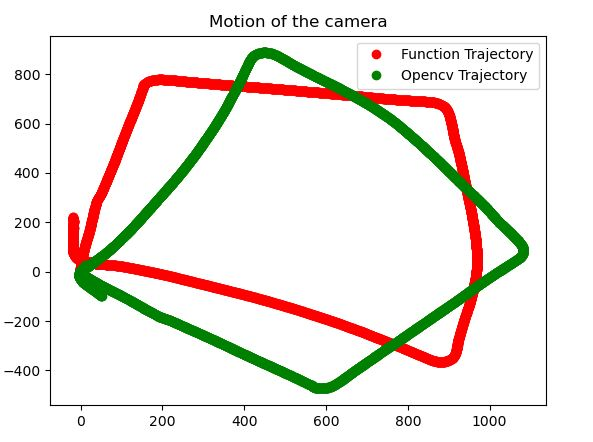
\includegraphics[width=11cm]{output2}
    \caption{Camera Trajectory comparison}
    \label{fig:Camera Trajectory comparison}
\end{figure}

\section{Output videos:}
To access the output video please click on this \href{https://drive.google.com/drive/folders/1bHtRRyyHCVfVULQ9rLM1Tsxr-f1liSLU?usp=sharing}{\underline{link}}.

\section{Team Members:}
1. Eashwar Sathyamurthy
2. Akwasi A Obeng
3. Achal P Vyas

\section{Difficulty faced:}
The RANSAC algorithm did not sample the points accurately. As a result, we got different values from the Opencv function. Due to large input data size, we ran the program for about half a day to get the output video.
\end{document}
